\section{Results}

Current results include the generation of time series data to be used in
training the RC model. Shown in Figure \ref{fig:demand}, Figure \ref{fig:solar}, and Figure \ref{fig:wind}.

\begin{figure}[h]
 	\centering
 	\label{fig:demand}
 	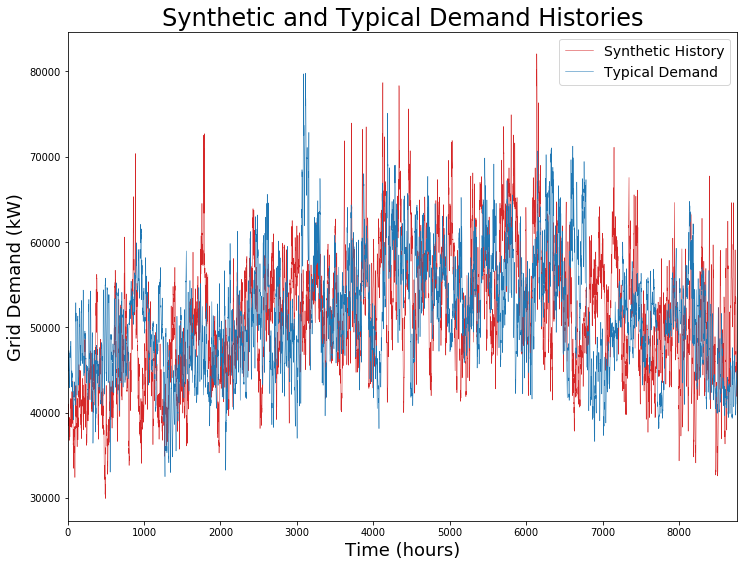
\includegraphics[width=0.8\columnwidth]{syn_typ_demand.png}
 	\caption{The typical year of hourly grid demand in kW at UIUC.}
\end{figure}
\begin{figure}[h]
	\centering
	\label{fig:solar}
	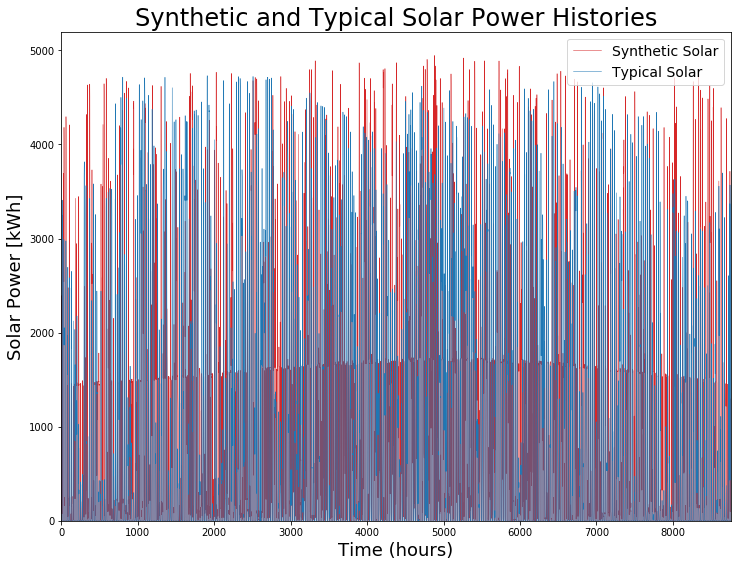
\includegraphics[width=0.8\columnwidth]{syn_typ_solar.png}
	\caption{The typical year and a synthetic year of hourly solar electricity
  generation in kWh per hour at UIUC. Data from
  \cite{alsoenergy_university_2019}}
\end{figure}
\begin{figure}[h]
	\centering
	\label{fig:wind}
	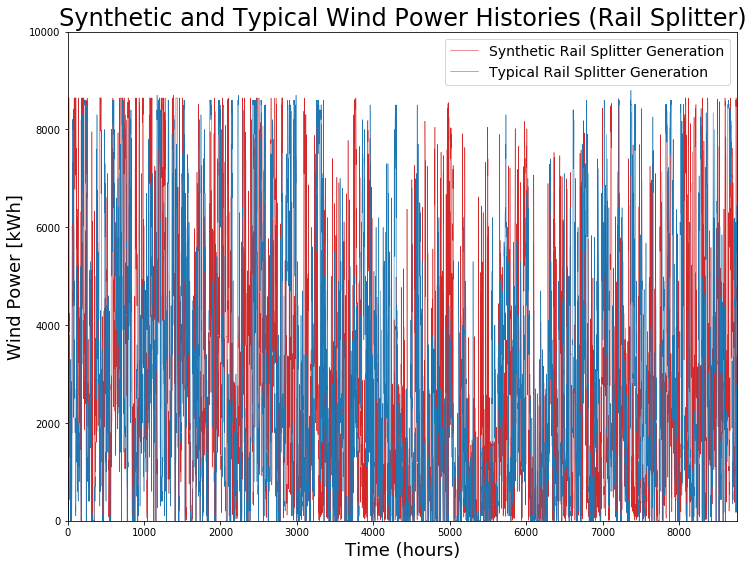
\includegraphics[width=0.8\columnwidth]{syn_typ_railsplitter.png}
	\caption{The typical year and a synthetic year of hourly power produced by
  the UIUC wind power purchase agreement with Railsplitter Wind Farm.}
\end{figure}

Additionally, preliminary predictions from a simple \acrshort{ESN}
in Figure \ref{fig:ESN1} and Figure \ref{fig:ESN2} show good fitness with grid
demand

\begin{figure}[h]
  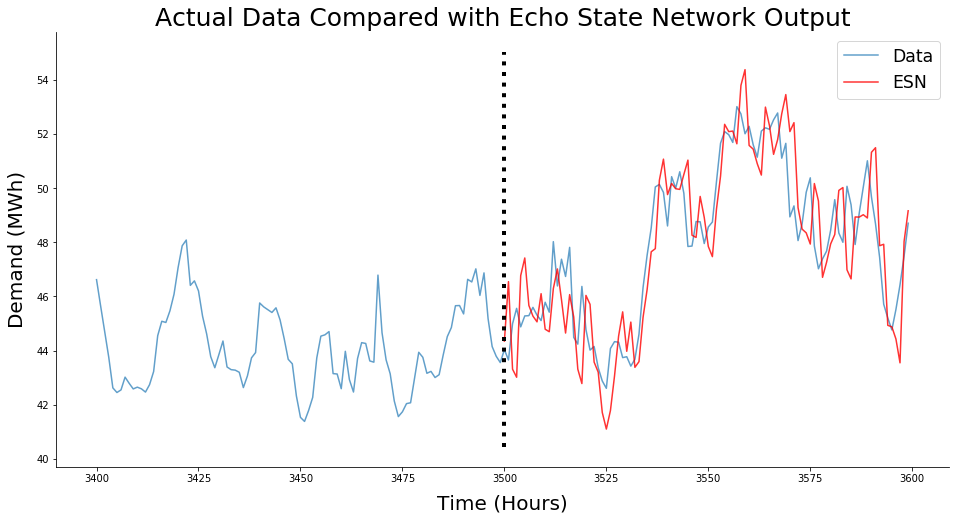
\includegraphics[width=\columnwidth]{scaled_esn_network.png}
  \caption{A simple ESN with a prediction of 100 hours into the future.}
  \label{fig:ESN1}
\end{figure}
\begin{figure}[h]
  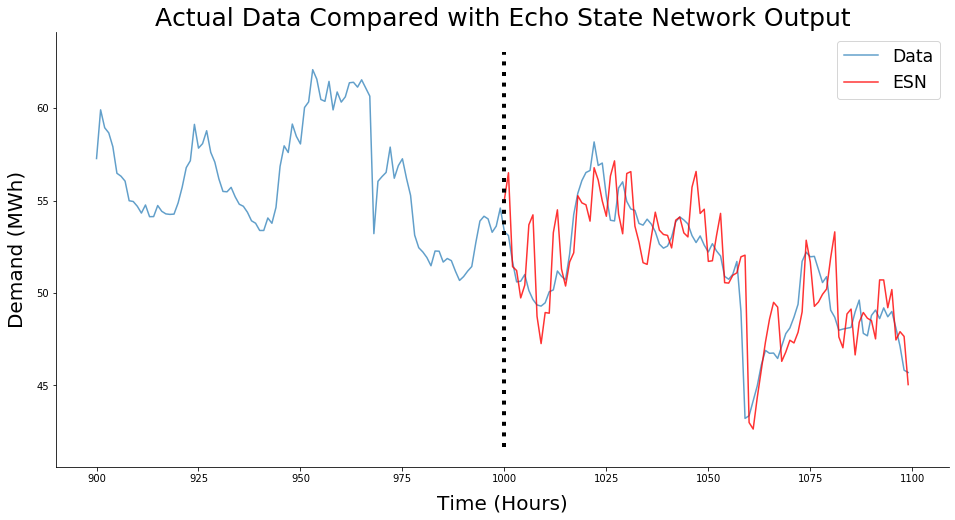
\includegraphics[width=\columnwidth]{scaled_esn_network2.png}
  \caption{A simple ESN with a prediction of 100 hours into the future.}
  \label{fig:ESN2}
\end{figure}
